\documentclass[a4paper,11pt]{article}

\usepackage[utf8]{inputenc}

\usepackage{minted}
\usepackage{graphicx}
\usepackage{placeins}

\begin{document}


\title{
    \textbf{Tree report}
}
\author{Jonathan Karlsson}
\date{Fall 2023}

\maketitle

\section*{Introduction}
This assignment involved creating a binary tree, creating and benchmarking methods for the tree aswell as creating an iterator for the tree.
\section*{Implementation}
The first method that had to be implemented was the add method which adds an integer to the tree at the position specified by the key, if the key already exists the add method changes the value of the key instead of adding it again. 
The add method firsts checks if the root is null, if it is then change the root to a new node with the key and the value, this is done whenever the tree is empty. 
If the tree was not empty the add method goes through the tree until either the key was found or the bottom of the tree was reached. When going through the tree the method checks if the key is larger than or smaller than the current element, and chooses if it should 
continue right or left in the tree. If it was not larger or samller than it was the same and then the value of the node is changed. If the key was not found in the tree it is added and the previous node is set to point at it. 
\begin{minted}{java}
public void add(Integer key, Integer value) {
    if (root == null) {
        root = new Node(key, value);
    } 
    else {
        Node curr = root;
        boolean found = false;
        Node prev = null;
        while (curr != null && found == false) {
            if (curr.key < key) {
                prev = curr;
                curr = curr.right;
            }
            else if (curr.key > key) {
                prev = curr;
                curr = curr.left;
            }                
            else {
                prev = curr;
                curr.value = value;
                found = true;
            }
        }
        if (curr == null) {
                curr = new Node(key, value);
            if (curr.key < prev.key)
                prev.left = curr;
            else
                prev.right = curr;
        }
    }
}
\end{minted}
The second method lookup was implemented in a similar way as add except for the fact that if the key was not found, instead of adding it lookup returns null and if it was found lookup returns its value.
\begin{minted}{java}
public Integer lookup(Integer key) {
    if (root == null) {
        return null;
    }     
    else {
        Node curr = root;
        while (curr != null) {
            if (curr.key < key) {
                curr = curr.right;
            }             
            else if (curr.key > key) {
                curr = curr.left;
            }             
            else {
                return curr.value;
            }
        }
        return null;
    }  
}
\end{minted}
\subsection*{Iterator}
As most if the most for the iterator was already given in the assignment, the only parts that had to be written were the contstructor, the hasNext and the Next method.
The contstructor for the iterator was pretty simple. It takes the root for the tree as an argument and saves it, then it starts from the root and goes as far to the left as possible with the next pointer while pushing to the stack, this is as the first element will be the object as far to the left as possible from the root.
\begin{minted}{java}
public TreeIterator(Node root) {
    stack = new Stack<Node>();
    next = root;
    this.root = root;
    stack.push(next);
    if(next!=null){
        while (next.left!=null) {
            next = next.left;
            stack.push(next);
        }
    }
}
\end{minted}
The hasNext method was also simple, as the contstructor will find the next at the start and then the next method will find the next before returning the previous next, and if the next is null 
there is no next, therefore the hasNext only has to return if the next is not null.
\begin{minted}{java}
public boolean hasNext() {
    return next!= null;
}
\end{minted}
The final next method is the most complicated method as it has to move up and down the tree. It starts by popping from the stack and saving it as the returnNode. this is the node that contains the value that will be returned, then the method finds the next vlaue. 
This is done by first checking if it is possible to go right, this is possible if right is not null and if right is not the node that is supposed to be returned as then that node has already been checked. If it was possible to go right it goes one right by pushing then going right and then pushing again. Then the method again tries to go as far left as possible, to get the lowest value under this right node. 
If it was not possible to go right, the method instead tries going back, which is possible as long as next is not root. If it is possible to go back next is first backed once, then while it is still possible to back, which is chosen by a number of different conditions, such as that the next is not root, right is null or right is less or equal to the return and that next.key is not larger than the return key. 
When the next has moved back enough next gets pushed to the stack. Then finally before returnNode is returned a check to see if the whole tree has been checked is run, this happens if next is root and root is less than the retunNode or root doesn't have a right node. When this is true next is set to null, which means that has next will return false.
\begin{minted}{java}
public Integer next() {
    Node returnNode = stack.pop();
    if(next.right != null && next.right != returnNode){
        stack.push(next);
        next = next.right;
        stack.push(next);
        while (next.left!=null) {
            next = next.left;
            stack.push(next);
        }
    }
    else if(next.key!=root.key){
        next = stack.pop();
        while(next!=root&&(next.right==null||next.right.key<=returnNode.key)
        &&!(next.key>returnNode.key)){    
            next = stack.pop();
        }
        stack.push(next);
    }
    if(next == root && (root.key < returnNode.key||root.right==null))
        next = null;
    return returnNode.value;
}
\end{minted}
It seems that the iterator is able to handle if the tree is changed while it iterates, as if a new key value pair was added to the tree at a point further ahead than the iterator is currently while 
iterating it gets picked up, this is because the iterator only knows about the next object, so if a object is added after the next object the iterator will see it when it gets there.
\section*{Benchmark}
The benchmark for this assignment was to benchmark the lookup algorithm from the tree and compare it to a binary search from the previous assignment. 
When benchmarking the tree was filled with random keys, as if the keys were ordered the next key would always be to the right which would make the lookup really simple to run.
Table for the results can be found below.
\begin{table}[h]
    \begin{center}
    \scalebox{1}{
    \begin{tabular}{l|c|c|}
    \textbf{n} & \textbf{Search({\textmu}s)} & \textbf{Tree({\textmu}s)}\\
    \hline
    100   &  269 &       5\\
    200   &  328 &       5\\
    400   &  383 &      14\\
    800   &  428 &      39\\
   1600   &  488 &      93\\
   3200   &  532 &     220\\
   6400   &  579 &     539\\
  12800   &  635 &    1383\\
  25600   &  696 &    3436\\
  51200   &  757 &    7606\\
 102400   &  865 &   17065\\
 204800   &  995 &   49048\\


    \end{tabular}
    }
    \caption{The result of Binary tree comapred to binary search}
    \label{tab:table1}
    \end{center}
\end{table}
\FloatBarrier{\noindent}
It seems that the binary search is a better choice when searching through large data sets while a tree can be better at smaller data sets.
This can also be seen in the graph below.




\begin{figure}[h]
    \centering    
    
    \scalebox{0.8}{% GNUPLOT: LaTeX picture with Postscript
\begingroup
  \makeatletter
  \providecommand\color[2][]{%
    \GenericError{(gnuplot) \space\space\space\@spaces}{%
      Package color not loaded in conjunction with
      terminal option `colourtext'%
    }{See the gnuplot documentation for explanation.%
    }{Either use 'blacktext' in gnuplot or load the package
      color.sty in LaTeX.}%
    \renewcommand\color[2][]{}%
  }%
  \providecommand\includegraphics[2][]{%
    \GenericError{(gnuplot) \space\space\space\@spaces}{%
      Package graphicx or graphics not loaded%
    }{See the gnuplot documentation for explanation.%
    }{The gnuplot epslatex terminal needs graphicx.sty or graphics.sty.}%
    \renewcommand\includegraphics[2][]{}%
  }%
  \providecommand\rotatebox[2]{#2}%
  \@ifundefined{ifGPcolor}{%
    \newif\ifGPcolor
    \GPcolortrue
  }{}%
  \@ifundefined{ifGPblacktext}{%
    \newif\ifGPblacktext
    \GPblacktextfalse
  }{}%
  % define a \g@addto@macro without @ in the name:
  \let\gplgaddtomacro\g@addto@macro
  % define empty templates for all commands taking text:
  \gdef\gplbacktext{}%
  \gdef\gplfronttext{}%
  \makeatother
  \ifGPblacktext
    % no textcolor at all
    \def\colorrgb#1{}%
    \def\colorgray#1{}%
  \else
    % gray or color?
    \ifGPcolor
      \def\colorrgb#1{\color[rgb]{#1}}%
      \def\colorgray#1{\color[gray]{#1}}%
      \expandafter\def\csname LTw\endcsname{\color{white}}%
      \expandafter\def\csname LTb\endcsname{\color{black}}%
      \expandafter\def\csname LTa\endcsname{\color{black}}%
      \expandafter\def\csname LT0\endcsname{\color[rgb]{1,0,0}}%
      \expandafter\def\csname LT1\endcsname{\color[rgb]{0,1,0}}%
      \expandafter\def\csname LT2\endcsname{\color[rgb]{0,0,1}}%
      \expandafter\def\csname LT3\endcsname{\color[rgb]{1,0,1}}%
      \expandafter\def\csname LT4\endcsname{\color[rgb]{0,1,1}}%
      \expandafter\def\csname LT5\endcsname{\color[rgb]{1,1,0}}%
      \expandafter\def\csname LT6\endcsname{\color[rgb]{0,0,0}}%
      \expandafter\def\csname LT7\endcsname{\color[rgb]{1,0.3,0}}%
      \expandafter\def\csname LT8\endcsname{\color[rgb]{0.5,0.5,0.5}}%
    \else
      % gray
      \def\colorrgb#1{\color{black}}%
      \def\colorgray#1{\color[gray]{#1}}%
      \expandafter\def\csname LTw\endcsname{\color{white}}%
      \expandafter\def\csname LTb\endcsname{\color{black}}%
      \expandafter\def\csname LTa\endcsname{\color{black}}%
      \expandafter\def\csname LT0\endcsname{\color{black}}%
      \expandafter\def\csname LT1\endcsname{\color{black}}%
      \expandafter\def\csname LT2\endcsname{\color{black}}%
      \expandafter\def\csname LT3\endcsname{\color{black}}%
      \expandafter\def\csname LT4\endcsname{\color{black}}%
      \expandafter\def\csname LT5\endcsname{\color{black}}%
      \expandafter\def\csname LT6\endcsname{\color{black}}%
      \expandafter\def\csname LT7\endcsname{\color{black}}%
      \expandafter\def\csname LT8\endcsname{\color{black}}%
    \fi
  \fi
    \setlength{\unitlength}{0.0500bp}%
    \ifx\gptboxheight\undefined%
      \newlength{\gptboxheight}%
      \newlength{\gptboxwidth}%
      \newsavebox{\gptboxtext}%
    \fi%
    \setlength{\fboxrule}{0.5pt}%
    \setlength{\fboxsep}{1pt}%
    \definecolor{tbcol}{rgb}{1,1,1}%
\begin{picture}(7200.00,5040.00)%
    \gplgaddtomacro\gplbacktext{%
      \csname LTb\endcsname%%
      \put(1210,704){\makebox(0,0)[r]{\strut{}$1$}}%
      \put(1210,1390){\makebox(0,0)[r]{\strut{}$10$}}%
      \put(1210,2076){\makebox(0,0)[r]{\strut{}$100$}}%
      \put(1210,2762){\makebox(0,0)[r]{\strut{}$1000$}}%
      \put(1210,3447){\makebox(0,0)[r]{\strut{}$10000$}}%
      \put(1210,4133){\makebox(0,0)[r]{\strut{}$100000$}}%
      \put(1210,4819){\makebox(0,0)[r]{\strut{}$1\times10^{6}$}}%
      \put(1342,484){\makebox(0,0){\strut{}$100$}}%
      \put(2707,484){\makebox(0,0){\strut{}$1000$}}%
      \put(4073,484){\makebox(0,0){\strut{}$10000$}}%
      \put(5438,484){\makebox(0,0){\strut{}$100000$}}%
      \put(6803,484){\makebox(0,0){\strut{}$1\times10^{6}$}}%
    }%
    \gplgaddtomacro\gplfronttext{%
      \csname LTb\endcsname%%
      \put(209,2761){\rotatebox{-270}{\makebox(0,0){\strut{}time in µs}}}%
      \put(4072,154){\makebox(0,0){\strut{}n}}%
      \csname LTb\endcsname%%
      \put(2266,4646){\makebox(0,0)[r]{\strut{}Search}}%
      \csname LTb\endcsname%%
      \put(2266,4426){\makebox(0,0)[r]{\strut{}Tree}}%
      \csname LTb\endcsname%%
      \put(2266,4206){\makebox(0,0)[r]{\strut{}log(n)}}%
      \csname LTb\endcsname%%
      \put(2266,3986){\makebox(0,0)[r]{\strut{}n}}%
    }%
    \gplbacktext
    \put(0,0){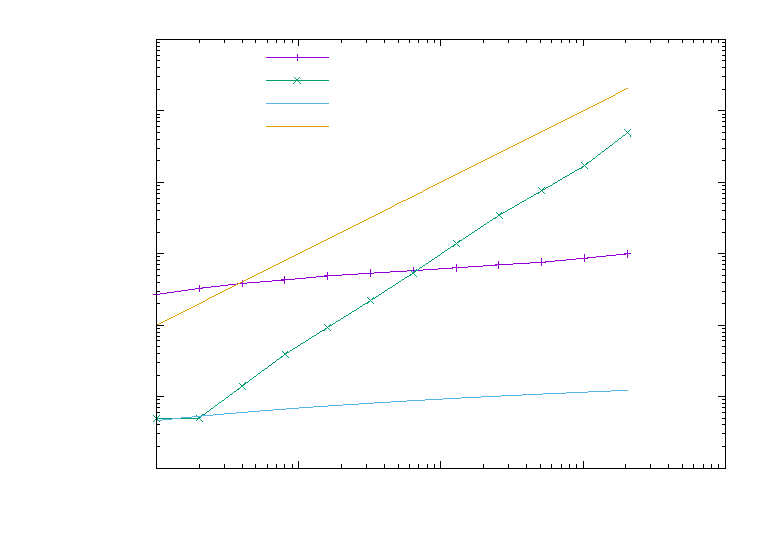
\includegraphics[width={360.00bp},height={252.00bp}]{disp}}%
    \gplfronttext
  \end{picture}%
\endgroup
}
    \caption{Visualization of BinarySearch and BinaryTree}   
    \label{tab:figure1} 
    
    \end{figure}
\noindent
Here it is possible to see that binary search is $O(log(n))$, while the tree seems to be more of $O(n)$. which was also evident in the previous table as for each time the elements increased by 2 times the previous elements, the time of the tree increased by around 2.3 times the previous time.


\end{document}
